\documentclass[portuguese]{textolivre}

% metadata
\journalname{Texto Livre}
\thevolume{18}
%\thenumber{1} % old template
\theyear{2025}
\receiveddate{\DTMdisplaydate{2024}{7}{18}{-1}}
\accepteddate{\DTMdisplaydate{2024}{10}{9}{-1}}
\publisheddate{\today}
\corrauthor{Daiane Padula Paz}
\articledoi{10.1590/1983-3652.2025.53547}
%\articleid{NNNN} % if the article ID is not the last 5 numbers of its DOI, provide it using \articleid{} commmand 
% list of available sesscions in the journal: articles, dossier, reports, essays, reviews, interviews, editorial
\articlesessionname{articles}
\runningauthor{Paz et al.}
%\editorname{Leonardo Araújo} % old template
\sectioneditorname{Daniervelin Pereira}
\layouteditorname{Leonardo Araújo}

\title{Entre fatos e relatos: as dimensões da identidade profissional e da competência digital docente}
\othertitle{Between facts and narratives: the dimensions of professional identity and digital competence of educators}

\author[1,2]{Daiane Padula Paz~\orcid{0000-0003-2658-9426}\thanks{Email: \href{mailto:daippaz@gmail.com}{daippaz@gmail.com}}}
\author[1]{Edilson Pontarolo~\orcid{0000-0002-6382-6403}\thanks{Email: \href{mailto:epontarolo@utfpr.edu.br}{epontarolo@utfpr.edu.br}}}
\author[3]{Rosa Vazquez Recio~\orcid{0000-0001-6595-177X}\thanks{Email: \href{mailto:rmaria.vazquez@gm.uca.es}{rmaria.vazquez@gm.uca.es}}}
\author[1]{Franciele Clara Peloso~\orcid{0000-0002-9647-001X}\thanks{Email: \href{mailto:clara@utfpr.edu.br}{clara@utfpr.edu.br}}}
\affil[1]{Universidade Tecnológica Federal do Paraná, campus Pato Branco, PR, Brasil.}
\affil[2]{Instituto Federal do Paraná, campus Palmas, PR, Brasil.}
\affil[3]{Universidade de Cádiz, campus Puerto Real, Espanha}

\addbibresource{article.bib}

\begin{document}
\maketitle
\begin{polyabstract}
\begin{abstract}
A Identidade Profissional e a Competência Digital Docente são dois temas importantes na área da Educação e que são pouco relacionados na literatura. Por seu ineditismo, delineou-se este artigo que tem por objetivo apresentar e descrever três dimensões de análise referentes à Identidade Profissional e à Competência Digital docente. Classifica-se metodologicamente como pesquisa biográfico-narrativa, uma vez que recorre a histórias de vida de quatro docentes de uma instituição pública do Brasil, para aproximar-se de seus percursos, experiências e inquietudes e de como se interrelacionam e se complementam. As aproximações realizadas entre o marco teórico mobilizado e os relatos dos docentes permitiram elucidar aspectos do fazer pedagógico que podem impactar na Identidade Profissional e na Competência Digital Docente e vice-versa. Entre as contribuições dessa pesquisa está o valor conferido às narrativas de trajetórias e vivências singulares desses profissionais da Educação, como instrumento para refletir sobre si e partilhar saberes que favorecem o seu próprio desenvolvimento pessoal, digital e profissional.

\keywords{Identidade profissional \sep Competência digital \sep Narrativas}
\end{abstract}

\begin{english}
\begin{abstract}
Professional Identity and Digital Competence of Educators are two important topics in the field of Education that are little related in the literature. Due to its originality, this article was outlined with the objective of presenting and describing three dimensions of analysis related to the professional identity and digital competence of Educators. Methodologically framed as biographical-narrative research, it draws on the life stories of four teachers from a public institution in Brazil, as a way of approaching their journeys, experiences, and concerns, and how they interrelate and complement each other. The connections made between the theoretical framework mobilized and the educators’ accounts made it possible to clarify aspects of pedagogical practice that affect professional identity and digital competence of educators and vice versa. Among the contributions of this research is the value sited on the narratives of the trajectories and unique experiences of these education professionals, as an instrument for self-reflection and sharing knowledge that favors their own personal, digital, and professional development.

\keywords{Professional identity \sep Digital competence \sep Narratives}
\end{abstract}
\end{english}
\end{polyabstract}

\section{Introdução}
A Identidade Profissional e a Competência Digital Docente são dois temas importantes na área da Educação e que são pouco relacionados entre si na literatura acadêmica. Dada sua relevância, desenvolveu-se este artigo, que é um recorte da tese intitulada “Entre-nós”: A urdidura da identidade profissional e da competência digital docente” \cite{paz2023}, o qual tem por objetivo apresentar e descrever três dimensões de análise referentes à Identidade Profissional e à Competência Digital Docente em que o estudo se apoiou e que se configuraram como achados da pesquisa, a saber: Dimensão 1 - A Identidade Profissional: Reconstruindo o caminho para a docência; Dimensão 2 - Ser docente na atualidade: demandas e crise; Dimensão 3 - Competência Digital Docente: autopercepção. Caracterizada metodologicamente como pesquisa de caráter qualitativo, com enfoque biográfico-narrativo, este estudo teve como instrumento uma entrevista biográfica, realizada com quatro docentes de uma instituição de ensino da Rede Federal de Educação Profissional, Científica e Tecnológica do sul do Brasil.

Este artigo apresenta a introdução, com a apresentação geral do texto ao leitor; o percurso metodológico, seção que descreve procedimentos do marco metodológico e teórico da pesquisa que deu origem aos três grandes eixos temáticos, denominados como dimensões; e uma terceira seção, denominada “Entre fatos e relatos: As dimensões da Identidade Profissional e da Competência Digital Docente”, a qual, subdividida em outras três subseções, descreve os objetivos de cada dimensão e as percepções obtidas a partir das experiências e narrativas docentes, o que justifica o título desse artigo. A seção final, “De aproximações a contribuições: O devir da pesquisa”; descreve aproximações que transitam entre o individual e o coletivo profissional docente e sintetiza as contribuições dessa pesquisa no campo da Educação.

\section{Percursos metodológicos}\label{sec-normas}
Na revisão de literatura sobre Competência Digital Docente (CDD), realizada por \textcite{paz2022}, identificou-se que uma parcela significativa de estudos publicados sobre essa temática tem enfoque em avaliar e categorizar esse construto em níveis de domínio, numa matriz fechada e homogênea, na maioria das vezes, com uma tendência quantificável. Entende-se, porém, que existem casos em que as metodologias convencionais, com uma perspectiva fechada, não são suficientes, ou mesmo ideais, para abarcar as especificidades de temas subjetivos ou complexos, deixando lacunas de natureza causal, contextual, social e epistemológica. Por esse motivo, surgiu o interesse de investigar a CDD em uma perspectiva abrangente, que possibilitasse aproximar-se das possíveis relações entre fatores e vivências que se justapõem no seu desenvolvimento e que afetam ou são afetados pela Identidade Profissional Docente (IPD).

Caracterizada metodologicamente como pesquisa de caráter qualitativo, com enfoque biográfico-narrativo, teve como instrumento central uma entrevista biográfica, a qual, segundo \textcite{bolivar1998}, oportuniza aos participantes recontar sua história de vida a partir de questões temáticas. Realizadas com quatro docentes de uma instituição da Rede Federal de Educação Profissional, Científica e Tecnológica, as entrevistas individuais orbitaram sobre três grandes eixos temáticos que conjugam elementos da Identidade Profissional Docente, da Competência Digital Docente e fatores e vivências da trajetória de vida, denominados neste estudo como dimensões (\Cref{fig1}).

\begin{figure}
    \centering
    \begin{minipage}{.75\textwidth}
    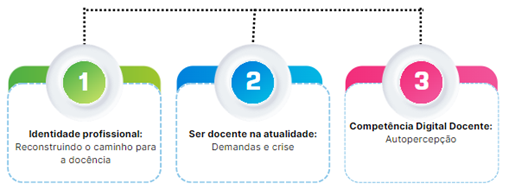
\includegraphics[width=\linewidth]{Figura1.png}
    \caption{Dimensões da pesquisa.}
    \label{fig1}
    \source{Elaborado pelos autores.}
    \end{minipage}
\end{figure}

As entrevistas se deram em três encontros, cada um pautado em uma das dimensões estipuladas previamente. Não foi estipulado tempo duração, tampouco questões fechadas, apenas um guia com os tópicos a serem tratados, considerados elementos das dimensões (\Cref{fig2}). Por ser uma entrevista em profundidade, a intenção era de uma fala livre por parte dos participantes e uma escuta intencionada por parte do pesquisador, com intervenção mínima, apenas para compreender as formas de sentir e se desenvolver na profissão de cada um. Com essa postura horizontal, tentou-se não reproduzir uma pesquisa de cima para baixo, que domina e “dá voz” \cite{vazquezrecio2022}, mas expressar um gesto metodológico que escuta, efetivamente, quem tem muito a dizer; nesse caso, os docentes. 

Todas as entrevistas foram transcritas, formando um corpus linguístico que foi analisado à luz do método Análise de Conteúdo, de \textcite{bardin2016}, cujos índices e referências foram estipulados a priori e codificados no software Atlas.ti. O confronto dos relatos e do referencial teórico consultado permitiram identificar aspectos que impactam na IPD e na CDD, cujas aproximações estão descritas na seção quarta deste artigo.

No que tange à construção da identidade, enfoque da Dimensão 1, oportunizada pelo exercício biográfico, o estudo baseou-se no que \textcite{dubar2005} define como uma transação dupla, em que a via biográfica revela o que o sujeito foi e/ou deseja ser, e a via relacional destaca os contextos em que se insere. Acatando esse posicionamento, o instrumento de entrevista foi elaborado como meio para a reflexão sobre o passado, a partir da rememoração do caminho para a docência, para a consciência do momento presente, com enfoque na instituição em que os docentes atuam e, ainda, para identificar as perspectivas de futuro na profissão.

Ao tratar de aspectos relacionados ao que representa ser docente na atualidade, tema central da Dimensão 2, foi considerado como os participantes declaram sentir-se para atender as gerações atuais, com ênfase em suas maiores dificuldades e necessidades formativas, experiências que lhes marcaram positivamente ou não, relações com a comunidade escolar e, especialmente, os sintomas de crise profissional \cite{bolivar2006}, não apenas pelas condições de precariedade em que muitos trabalham, mas pelas mudanças advindas da expansão das Tecnologias da Informação e Comunicação, as quais se intensificaram ainda mais no período da pandemia da Covid-19.

No que tange à Dimensão 3, cujo enfoque foi a autopercepção sobre a Competência Digital Docente, a pesquisa não teve por intenção reforçar a tendência de mensurar o perfil docente sobre o uso de recursos tecnológicos, embora entenda a importância das escalas da CDD elaboradas por pesquisadores da área. Primou-se por elencar elementos em comum na rede de categorias das áreas de avaliação dispostas no European Framework for the Digital Competence for Educators: DigCompEdu \cite{redecker2017}, que permeiam o fazer docente e revelam idiossincrasias e coletividades. Pretendeu-se, dessa forma, compreender como o docente se constitui ao longo de sua trajetória profissional e como o digital pode modificar sua IPD. 

\section{Entre fatos e relatos: as dimensões da identidade profissional e da competência digital docente}\label{sec-fmt-manuscrito}
Como já mencionado, a pesquisa realizada sentou bases em dois grandes temas: a Identidade Profissional e a Competência Digital Docente. Desses temas, advieram as três dimensões de análise, as quais, baseadas na literatura consultada, contemplaram diversos elementos (\Cref{fig2}) que fundamentaram os roteiros de cada uma das sessões das entrevistas.

\begin{figure}
    \centering
    \begin{minipage}{.75\textwidth}
    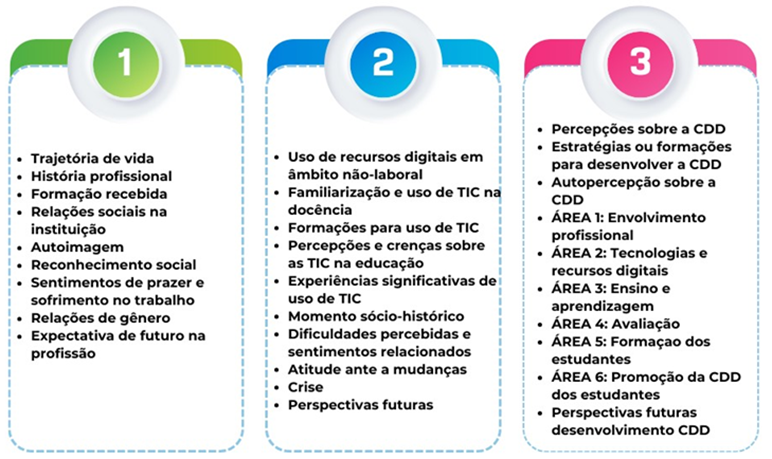
\includegraphics[width=\linewidth]{Figura2.png}
    \caption{Elementos das dimensões de análise.}
    \label{fig2}
    \source{\textcite{paz2023}.}
    \end{minipage}
\end{figure}

\subsection{Dimensão 1 − Identidade profissional: reconstruindo o caminho para a docência }\label{sec-formato}
O eixo temático da primeira dimensão foi a Identidade Profissional dos docentes. A intenção desse roteiro foi acercar-se dos percursos individuais dos docentes participantes da pesquisa, buscando conhecer dados de sua trajetória de vida e de formação, especialmente no que se refere aos processos de escolha da profissão docente, suas expectativas, influências recebidas, como se deu a estreia na profissão e, ainda, sobre suas relações na instituição onde trabalham atualmente. Com esse repertório de caráter subjetivo, foi possível fomentar relatos pessoais, com vistas à compreensão de cada um sobre si mesmo, ou seja, suas histórias de emancipação \cite{rivas2011}.

Também nesse roteiro foram inseridos os elementos que \textcite{bolivar2006} destaca como essenciais para a construção da referida identidade, a saber: autoimagem; reconhecimento social; relações de prazer e sofrimento; relações sociais na instituição; atitude ante a mudança; competências profissionais; expectativas de futuro na profissão. Além desses, a pesquisadora adicionou ainda outros dois aspectos considerados importantes: as relações de gênero e o momento sócio-histórico. 

Esta dimensão inicial foi elaborada cuidadosamente para promover um processo reflexivo inicial, cheio de significados, designado por \textcite{josso2004} como o “caminho para si”, e que representa:

\begin{quote}
    um projeto à escala de uma vida, cuja atualização consciente passa, em primeiro lugar, pelo projeto daquilo que somos, que pensamos, que fazemos, que valorizamos e que desejamos na nossa relação conosco, com os outros e com o meio humano e natural \cite[p.~43]{josso2004}.
\end{quote}

Ainda que os históricos permitam de obter uma visão estática “original” de si, vale lembrar que a identidade “é um significado cultural e socialmente atribuído” \cite[p.~89]{silva2020}, ao mesmo tempo singular e múltiplo, que se modifica continuamente, associada ao momento em que a sociedade se encontra \cite{bauman2021,hall2000,hall2020}. Por esse motivo, as entrevistas não se deram de igual forma com cada participante, uma vez que pelos próprios temas dos roteiros, outros pontos vinham à tona, enriquecendo ainda mais as manifestações singulares nas narrativas.

\subsection{Dimensão 2 − Ser docente na atualidade: demandas e crise}\label{sec-modelo}
A Dimensão 2, Ser docente na atualidade: demandas e crise, teve por intenção retomar aspectos que podem ter contribuído para a construção da Identidade Profissional dos docentes, dando enfoque em aspectos relacionados às demandas da atualidade. Nesse roteiro, os participantes foram incitados a relatar sobre seu percurso de formação, seu processo de familiarização com recursos digitais, suas experiências pedagógicas e dificuldades sentidas, tanto em relação ao uso de tecnologias quanto com a geração atual, que são seus alunos. Também foi retomado o contexto da pandemia da Covid-19 por considerá-lo um incidente crítico, que para \textcite{bolivar2006}, são como motores de mudança na trajetória de vida de cada um.

Nesta dimensão, o tema crise de identidade \cite{dubar2009,hall2020} foi abordado continuamente, dado que o indivíduo da atualidade tem sentido os efeitos das profundas transformações de uma sociedade cada vez mais globalizada, fragmentada e hibridizada, conforme afirmam \textcite{giddens2002,bauman2021}. Ao tratar das demandas da atualidade buscou-se elencar as percepções dos docentes sobre as mudanças ocasionadas pela crescente expansão das Tecnologias Digitais de Informação e Comunicação (TDICs) no campo da Educação e, também, como se sentiram na implementação do ensino remoto durante o período da pandemia, além das considerações sobre como percebem a profissão atualmente.

Em contraposição à crise profissional e suas agruras, buscou-se reavivar na memória dos docentes experiências significativas de sua trajetória profissional incluindo ou não o uso de tecnologias, ocasiões em que se sentiram ou que lhes fazem sentir contentes no seu trabalho, incluindo satisfação e reconhecimento profissional. Por fim, com vistas ao futuro na profissão, buscou-se conhecer as projeções e desejos de cada docente para os próximos anos. Assim, pelas nuances de retrospeção e de projeção, conformou-se a (re)construção da identidade profissional como meio de reafirmação de si e do seu papel na sociedade, resgatando internamente o valor da profissão.

\section{Dimensão 3 − Competência digital docente: autopercepção}\label{sec-organizacao}
A Dimensão 3, Competência Digital Docente: autopercepção, foi elaborada para conhecer aspectos específicos da CDD, centrando-se na percepção dos participantes sobre esse construto e reflexão sobre suas habilidades no entorno digital. Assim, o roteiro desta entrevista foi elaborado com base nos princípios do Quadro Comum Europeu de Referência para a Competência Digital \cite{punie2013} e assentado nas seis áreas para Avaliação de Competência Digital Docente do modelo DigiCompuEdu \cite{redecker2017} e na proposta de \textcite{trindade2019}, a saber: Área 1: Envolvimento Profissional; Área 2: Tecnologias e Recursos Digitais; Área 3: Ensino e Aprendizagem; Área 4: Avaliação; Área 5: Formação dos Estudantes; Área 6: Promoção da Competência Digital dos Estudantes. O referencial teórico que dá suporte à construção dos elementos dessa dimensão foi selecionado na revisão de literatura sobre o tema, elaborada por \textcite{paz2022}.

Além dos elementos acima citados, adicionou-se como fechamento do roteiro dessa dimensão um item sobre as perspectivas futuras dos docentes em relação ao desenvolvimento de sua CDD. Desejava-se, dessa forma, conhecer suas necessidades de formação nesse campo, bem como suas intenções e áreas de interesse que relacionam o uso de tecnologias na Educação.

Cabe destacar que não houve neste estudo a intenção de avaliar habilidades ou compor um perfil dos participantes em relação aos níveis de sua CDD, mas sim promover reflexões sobre sua relação e uso das TDICs na prática docente, identificando fortalezas e debilidades nas diferentes áreas e, quando possível, os impactos no fazer-pedagógico de cada um.

\section{De aproximações a contribuições: o devir da pesquisa}\label{sec-organizacao-latex}
Os caminhos epistêmicos percorridos pela pesquisa empreendida permitiram lançar luz nas três dimensões já referidas – Identidade Profissional, Ser docente na atualidade, Competência Digital Docente –, e realizar algumas aproximações que transitam entre o individual e o coletivo docente, configurando aspectos pedagógicos que exercem influência na IPD e na CDD, conforme descrito a seguir:

\textit{Dimensão 1 - Identidade profissional: Reconstruindo o caminho para a docência}: ao recompor a trajetória individual de vida e formação dos participantes e resgatar os motivos pelos quais escolheram a profissão docente, foi possível aproximar-se de rumos e aspectos individuais que forjaram a história de cada um. A retomada das expectativas iniciais e estreia na carreira, contrapondo com sua atuação profissional no presente, favoreceram a percepção de seus saberes experienciais e profissionais \cite{tardif2014}, e de todos os percursos que (re)modelaram seu fazer pedagógico com o passo do tempo. A consciência dos processos de socialização profissional \cite{dubar2012} e do crescimento intelectual e atitudinal também foi fomentada.

No acervo memorístico ativado de cada docente entrevistado fluíram relatos sobre como escolheram a profissão docente e sua respectiva área de atuação, as influências e desaprovações recebidas de pessoas próximas, bem como as expectativas e receios que sentiam no período de formação e no início de suas atividades profissionais. De forma longitudinal, do início à atualidade, conseguiram refletir sobre sua forma de atuar, perceber e sentir a profissão. Essa conformação expressada verbalmente e repleta de emoções e sensações genuínas, que vão desde desânimo pela falta de reconhecimento no trabalho exercido à orgulho por situações de êxito em práticas de sala de aula, legitimam a perspectiva de \textcite[p.~16]{pimenta1996} que declara que a identidade docente se constrói “pelo significado que cada professor, [...] confere à atividade docente no seu cotidiano com base em seus valores, seu modo de situar-se no mundo, suas histórias de vida, suas representações, seus saberes”.

O trabalho tem um importante papel na estruturação do indivíduo e, também, na promoção de prazer e/ou sofrimento \cite{codo1999}. Para os docentes, os sentimentos de satisfação e prazer se dão, essencialmente, pela evolução da aprendizagem de seus alunos, pelas boas relações e pelo reconhecimento de seu trabalho; enquanto o sofrimento se origina das condições laborais, que incluem precarização do trabalho, burocratização, falta de autonomia ou de boas parcerias para melhor desenvolvimento do trabalho, além de desvalorização econômica e social. Pelos relatos, percebeu-se que esses sentimentos reverberam diretamente em outros elementos da IPD elencados nesse estudo, como autoimagem, relações sociais na instituição, reconhecimento social e, inclusive, relações de gênero. 

 Ainda no que tange à identidade, pelas narrativas dos participantes, foi possível ratificar a percepção dos teóricos \textcite{dubar2005,bauman2021} de que ela se constrói de forma progressiva e contínua, e que nesse processo de movimento espiralado, os elementos constituintes da IPD elencados nesse estudo afetam uns aos outros. Por essa ótica, entende-se a unicidade e subjetividade do ser e que, por mais que professores tenham uma trajetória e/ou formação parecida, não exercerão a docência da mesma forma. Esse entendimento convalida a escolha metodológica dessa pesquisa e faz frente para outros estudos dessa natureza.
 
Também nessa dimensão, ao tratar das relações sociais estabelecidas na instituição onde trabalham, ficou evidente que existe uma identidade institucional que deve ser desenvolvida e valorizada no coletivo de cada unidade de ensino, pois favorece os sentimentos de pertença entre todos os componentes da comunidade escolar, o que pode qualificar o ensino através de ações colaborativas, corroborando o descrito por \textcite{bolivar2006} sobre a construção identitária enquanto fruto de uma relação entre si e os outros. Nesse sentido, a fala de um dos participantes sobre a sua satisfação em um dos locais em que trabalhava, ratifica: “E eu gostava muito de dar aula ali. Foi nessa escola que eu me identifiquei mesmo com a profissão” (Entrevista 1, Participante 2).

Como em todas as demais dimensões, o tópico final trata sobre expectativas, as quais representam “futuros estados ou situações desejadas que, com efeitos motivacionais, contribuem para dar energia e compromisso às situações presentes para consegui-las” \cite[p.~169]{bolivar1998}. Assim, no contraponto do recorrido no passado e com a intenção de fazer projeções sobre si mesmo na esfera pessoal e profissional, buscou-se saber como os docentes vislumbravam a profissão e o que desejam fazer futuramente. Os relatos foram um pouco pessimistas no sentido de que não imaginavam que a profissão seria tão difícil e que não possuem certeza de onde estarão no futuro, talvez porque por ser uma instituição federal com unidades espalhadas em todo o país, é comum haver pedidos de remoção para outros campi sobretudo por motivos pessoais. Por outro lado, todos os participantes declararam estar envolvidos em atividades de gestão e que possivelmente permanecerão, o que pode ser um indício de compromisso com a instituição e engajamento naquilo que fazem, reforçando sua identidade institucional.

\textit{Dimensão 2 - Ser docente na atualidade: demandas e crise}: os relatos sobre a docência na atualidade possibilitaram conformar os terrenos individuais e coletivos que os professores têm atravessado, evidenciando os processos de precarização da Educação e de descrédito social do ofício que favorecem o que \textcite{libaneo1998} denomina como desprofissionalização docente. Essa sensação de declínio, falta de autonomia, e de pouco reconhecimento no trabalho foi comum a todos os participantes, convertendo-se em questões importantes no campo da Educação, que devem ser consideradas para processos de reafirmação dessas identidades e, por conseguinte, valorização desses profissionais.

A dissociação entre a formação recebida e o que ocorre no cotidiano escolar, a angústia sobre como atender as demandas da atualidade, quer seja pelas diferenças de comportamentos e de interesses da geração atual, quer seja pela ausência de formações que contemplem as reais necessidades dos docentes, também foram apontadas pelos participantes. Identificou-se, porém, que existem esforços individuais para suprir suas lacunas, tanto com a ajuda entre pares de colegas, quanto com a realização de formações por conta própria, buscadas com maior urgência no período em que se instaurou o ensino remoto na instituição por conta do isolamento social no período de pandemia da Covid-19, e que revelam seus esforços individuais e coletivos para superar as dificuldades encontradas. Nessa perspectiva, a questão formativa que contemple a realidade local e das disciplinas ministradas foi uma demanda citada.

No cenário de mudanças constantes, o rechaço a novas habilidades, entre elas a CDD, pode ser entendido como um mecanismo para preservar a própria IPD ou a cultura escolar. Assim, o sentimento de insegurança expressado pelos docentes para inovar ou para incorporar recursos tecnológicos na sua prática docente é compreensível, afinal as mudanças afetam os conhecimentos, habilidades ou competências, além das dimensões afetivas e atitudinais \cite{bolivar2006}. 

A falta de estabilidade e valorização do ofício, por consequência de fatores sociais e políticos, gera entre seus principais agentes certa desorientação, interpretada por \textcite{esteve1999} como mal-estar docente. Esse sentimento ficou evidente em diversos relatos, demarcado por afirmativas pouco animadas sobre as condições de trabalho e pouco otimistas sobre futuras melhorias no panorama da Educação. Entretanto, com a evocação de memórias positivas a partir de experiências que lhe marcaram, os sentimentos de desconcerto, insegurança e angústia pareceram ser atenuados, dando espaço à esperança e desejo de ser melhor naquilo que faz. Esse movimento é benéfico porque permite o resgate daquilo que é essencial na profissão, como afeto, perseverança e envolvimento, os quais, junto com políticas educacionais e o redesenho de modos de pensar e fazer o ensino, poderão colaborar para processos de reconstrução identitária, conforme sugere \textcite{bolivar2006}. Isso pode ser percebido no seguinte relato de um dos docentes participantes da pesquisa:

\begin{quote}
    Eu penso que isso é uma crise, é um momento, é importante também a gente parar pra refletir. [...] E eu penso em mudar, eu penso em renovar, me renovar e tentar... eu vejo que esse ensino que eu pensava, que ia ser minha carreira de professor ia ser de uma forma, mas a sociedade muda e você precisa se renovar, se atualizar, precisa estudar... e é isso que eu quero, gosto ainda de ser professor (Entrevista 2, Participante 3).
\end{quote}

\textit{Dimensão 3 - Competência Digital Docente: autopercepção}: esta dimensão circundou de forma mais específica o tema Competência Digital Docente nas seis áreas do DigCompEdu \cite{redecker2017}. Na área 1: Envolvimento Profissional, os docentes evidenciaram sentir necessidade de maior interação entre os pares de colegas para intervenções pedagógicas conjuntas e, que embora façam esforços para esse fim, existem dificuldades de comunicação e de interesses comuns, além de uma tendência ao trabalho solitário, o que segundo \textcite{imbernon2017} agrava seu mal-estar. 

Na área 2, que trata sobre uso de tecnologias e recursos digitais, os docentes relataram fazer uma curadoria dos recursos a serem utilizados para verificar funcionalidades e se atendem os objetivos das atividades propostas. Entretanto, declaram sentir limitações tanto de disponibilidade de acesso, por usarem versões gratuitas, quanto de conhecimentos suficientes, o que segundo eles poderia ser sanado se houvesse maiores recursos e formações continuadas.

Na área 3: Ensino e aprendizagem, os relatos denotam que os participantes se preocupam em utilizar estratégias de ensino adequadas para os conteúdos, nível de ensino e faixa etária e condizentes com os recursos disponíveis, o que representa, para eles, um importante desafio. Destacam que o uso de ambientes virtuais antes da pandemia era esporádico, mas que durante e após o ensino remoto, tornou-se regular e importante.

A área 4, denominada Avaliação, tem por enfoque saber como são usadas as tecnologias digitais para melhorar os processos de avaliação dos estudantes. Esse aspecto pareceu ser uma debilidade comum entre os docentes, uma vez que relataram não conseguir utilizar como gostariam tais recursos, tentando avaliar progressivamente, mas não usando ferramentas que permitam acompanhar o desenvolvimento contínuo de seus estudantes. Na realidade, no tocante à avaliação da aprendizagem dos estudantes, segundo \textcite{sordi2009avaliacao} existe uma convergência entre docentes sobre sua complexidade, dado que na organização escolar existem diferentes atores, concepções e interesses. Sugere-se, portanto, que essa seja uma temática para uma formação organizada pelos gestores da instituição, de modo a suprir as necessidades pontuais do quadro docente, considerando o valor da avaliação enquanto categoria constitutiva de seu trabalho pedagógico.


A área 5, Formação dos estudantes, abrange a acessibilidade e inclusão, a diferenciação e personalização, e o envolvimento ativo dos estudantes \cite{lucas2018}. No que se refere à acessibilidade e inclusão, ficou evidente a presença de exclusão digital nos quatro níveis de acesso determinados por \textcite{vandijk2003} − acesso mental, acesso material, acesso a competências e acesso de uso – tanto entre docentes quanto discentes. Essa falta de equidade, que foi amplamente desvelada no período de ensino remoto é, com certeza, um ponto que necessita de urgente atenção por parte de políticas públicas, dado que a utilização de serviços digitais nas diferentes esferas e para os diversos fins é uma forma de participação social e, portanto, um direito humano. Ainda na área 5, outra debilidade encontrada foi a diferenciação e a personalização do ensino por parte dos docentes. Em seus relatos consideraram a dificuldade que sentem para adaptação de conteúdos e edição de materiais no entorno digital de forma que pudessem atender as necessidades individuais de cada aluno.

A área 6, que trata da promoção da Competência Digital dos estudantes, tem por objetivo possibilitá-los usar tecnologias digitais de forma criativa e responsável para informação, comunicação, criação de conteúdos, bem-estar e resolução de problemas \cite{lucas2018}. Nesse aspecto os docentes relataram que se preocupam com o uso ético e responsável das tecnologias por parte dos estudantes, sobretudo em redes sociais e grupos de mensagens instantâneas, fazendo alerta constante sobre comportamentos que não são saudáveis nesses ambientes. Relatam também que por dificuldades suas não conseguem favorecer que seus alunos resolvam problemas técnicos ou transfiram conhecimento tecnológico para outras situações, o que, nessa perspectiva, representa uma debilidade do docente que impacta no discente.

Além dos aspectos das seis áreas do DigCompEdu, nessa dimensão, foram fomentadas as percepções dos docentes sobre sua Competência Digital, suas estratégias de formação e perspectivas futuras para desenvolvê-la. Todos os participantes declararam que sentem algum tipo de limitação no entorno digital, e que isso, de certa forma, afeta seu desempenho ou expectativas na prática pedagógica cotidiana, portanto, têm buscado meios de autoformação (por videoaulas, cursos, ou ajuda entre colegas) que supram tais lacunas. 

Quanto às perspectivas futuras sobre o desenvolvimento de sua Competência Digital, os mesmos docentes destacaram que gostariam de realizar formações específicas para esse fim, mas que essas abrangessem suas áreas de atuação, possibilitando experiências práticas e eficazes do uso das TDICs para os conteúdos e disciplinas que ministram. 

Ainda sobre a relação dos docentes com as TDICs no uso educacional, os relatos revelaram a presença de sentimentos como insegurança, ansiedade e sensação de insuficiência, ou desatualização constante, conforme fica evidente no seguinte relato:

\begin{quote}
    [...] a gente estava até conversando sobre isso... porque dá medo de envelhecer e não acompanhar a evolução tecnológica. Não nesse sentido, por exemplo, dessas coisas de casa, que a gente não vai sentir necessidade; mas no trabalho... É possível que a gente fique ultrapassado. [...] Então eu acho que eu tenho medo de ficar desatualizada por não acompanhar esse processo de evolução e tudo mais. (Entrevista 2, Participante 3).
\end{quote}

Apesar das dificuldades, os docentes destacaram que existem benefícios do uso de TDICs nas aulas, resultando em maior interesse e engajamento por parte dos estudantes, assim como diferentes possibilidades de visualizar fenômenos (físicos ou biológicos, por exemplo); por esse motivo, afirmam que pretendem conhecer ainda mais recursos disponíveis para suas disciplinas e como usá-los para incrementar suas aulas. Esse aspecto configura-se também como uma expectativa de uso de Tecnologias na Educação.

Além de todos os pontos destacados em cada uma das três dimensões, que conformam uma perspectiva micro, cabe destacar algumas contribuições desse estudo numa perspectiva macro, que também configuram o seu devir, ou seja, seu percurso e ponto de chegada. Nesse sentido, a primeira contribuição trazida é o entrelaçamento de dois temas importantes no campo da Educação da atualidade − a Identidade Profissional Docente e a Competência Digital Docente − para o vislumbre de novas perspectivas de pesquisas. A segunda contribuição é a elaboração de uma matriz sistematizada em dimensões que contempla elementos desses dois temas centrais, que podem servir de base para estudos semelhantes em outros contextos. A terceira contribuição advém da perspectiva metodológica elegida para tratar o tema de CDD, que na perspectiva de biográfico-narrativa percebe a subjetividade como essencial e o participante como agente ativo \cite{miranda2019}, o que, além de favorecer o autoconhecimento sobre suas próprias habilidades e reflexão sobre suas debilidades, promove uma consciência histórica de cada um, reforça a importância de partilhar saberes experienciais em favor de novos modos de pensar e fazer a Educação e demarca uma abertura epistemológica de investigação na área \cite{souzaclementino2020}.

\section{Conclusão}\label{sec-titulo}
Esse artigo teve por objetivo apresentar e descrever três dimensões de análise referentes à Identidade Profissional Docente e à Competência Digital Docente em que o estudo se apoiou, a saber: Dimensão 1 - A Identidade Profissional: Reconstruindo o caminho para a docência; Dimensão 2 - Ser docente na atualidade: demandas e crise; Dimensão 3 - Competência Digital Docente: autopercepção. Tais dimensões foram descritas, considerando todos os elementos que as compõem, sustentadas no referencial teórico mobilizado na pesquisa.

As aproximações feitas entre a literatura e as narrativas dos docentes participantes trouxeram informações diversas sobre como a IPD é forjada dentro da cultura profissional e sobre como a própria relação dos docentes com as TDICs tem sido ponto de tensão quando aplicadas à Educação, colocando-os em autoquestionamento sobre seu valor, sua função na sociedade, além da necessidade novos conhecimentos, fomentando um novo viés da crise profissional do docente da atualidade. Por essa ótica, fica evidente que tecnologias têm afetado a IPD.

Esta pesquisa dá valor às narrativas de trajetórias e vivências singulares dos profissionais da Educação, como instrumento para refletir sobre si e partilhar saberes que favorecem o seu próprio desenvolvimento pessoal, digital e profissional, trazendo conhecimentos empíricos que confluem com os científicos. Essa perspectiva biográfica configura-se como uma nova forma para a compreensão mais profunda da CDD e seus impactos no fazer pedagógico.

Por ser um recorte de uma pesquisa de natureza mais ampla (tese), esse texto apresenta alguns pontos de forma sintética, o que pode ser considerada uma limitação, a qual pode ser sanada através da consulta da obra completa disponível nas referências.

\section{Agradecimentos}\label{sec-idioma}
À Fundação Carolina, pela bolsa de Mobilidade para Professores Brasileiros, concedida à autora principal no ano de 2021. Apoio que foi de extrema importância para o desenvolvimento desta pesquisa.

Ao Instituto Federal do Paraná, pelo Afastamento para Estudos, concedido durante parte desse estudo. Foi pela dedicação total à pesquisa que pude dar o melhor de mim.



\printbibliography\label{sec-bib}
%conceptualization,datacuration,formalanalysis,funding,investigation,methodology,projadm,resources,software,supervision,validation,visualization,writing,review
\begin{contributors}[sec-contributors]
\authorcontribution{Daiane Padula Paz}[conceptualization,datacuration,formalanalysis,investigation,methodology,writing]
\authorcontribution{Edilson Pontarolo}[conceptualization,projadm,methodology,projadm,visualization,review]
\authorcontribution{Rosa Vazquez Recio}[methodology,review]
\authorcontribution{Franciele Clara Peloso}[methodology,review]
\end{contributors}
\end{document}
